%$$\zeta (s) = \sum\limits_{n=1}^{\infty} \frac{1}{n^s},\,s = \sigma + it$$
%сходится при $\sigma > 1$
%$$-\frac{\zeta '(s)}{\zeta (s)} = O(\sqrt{t})$$
%при $\sigma > 1$ существует разложение
%$$-\frac{\zeta '(s)}{\zeta (s)} = \sum\limits_{n=1}^{\infty}\frac{\Lambda (n)}{n^s}$$
%где
%$$
%  \Lambda (n) =
%  \begin{cases}
%    \ln p, &n = p^k \\
%    0, &\text{иначe}
%  \end{cases}
%$$
%$$\psi(x) = \sum\limits_{n\leqslant x} \Lambda (n)$$
%Задача~--- доказать асимптотический закон $\pi (x) \sim \frac{x}{\ln x}$, что означает
%$$\lim\limits_{x \rightarrow + \infty} \frac{\pi (x) \ln x}{x}=1.$$\par
%Напомним, что
%$$\pi (x) \sim \frac{x}{\ln x} \Leftrightarrow \psi(x) \sim x, x\rightarrow + \infty,$$где
%$$\omega (x) = \int\limits_1^x \frac{\psi(t)}{t}\,dt$$
\subsection{Асимптотический закон}
\subsubsection{Функция $\om(x)$. Достаточность эквивалентности $\om(x)\sim x$ 
							для доказательства асимптотического закона}

Напомним, что мы доказали совпадение верхних и нижних пределов у функций 
$\frac{\psi(x)}{x}$ и $\frac{\pi(x)\ln{x}}{x}$, поэтому для доказательства
асимптотического закона $\pi(x)\sim\frac{x}{\ln{x}}$ достаточно показать,
что $\psi(x)\sim~x$.

Введем функцию 
$$
	\om(x):=\intlim_1^x \frac{\psi(t)}t\,dt.
$$

\begin{stm}
Если $\omega(x) \sim x$, то $\psi(x) \sim x$.
\end{stm}
\begin{note}
Верно и обратное утверждение, но нам достаточно этого.
\end{note}
\begin{proof}
Возьмем $u > v \geqslant 1$ и рассмотрим
$$
	\int\limits_v^u \frac{\psi(t)}{t}\,dt =\omega(u) - \omega(v) = 
	u - v + o(u) + o(v).
$$

Оценим его грубо сверху и снизу:
$(u-v)\frac{\psi(v)}{u} \leqslant \int\limits_v^u \frac{\psi(t)}{t}\,dt 
\leqslant (u-v)\frac{\psi(u)}{v}.$

Рассмотрим две ситуации:
\begin{points}{0}
\item Выберем $v = x,\,u = (1+\ep)x$, тогда имеем 
	$\ep x\frac{\psi(x)}{(1+\ep)x} \leqslant \ep x + o(x),$
	откуда $\psi(x) \leqslant (1+\ep)x + o(x)$, и найдется $x_1$ такой, 
	что при $x>x_1$ $\psi(x)\le(1+2\ep)x$.

\item Теперь возьмем $u = x,\,v = (1 - \ep)x$ и используем правую оценку: 
	$\ep x + o(x) \le \ep x\frac{\psi(x)}{(1-\ep)x}$, откуда аналогично \pt{1} 
	получаем, что при $x>x_2$ $\psi(x)\ge(1-2\ep)x$.

	Таким образом, при $x>\max{(x_1,\,x_2)}$ имеем
	$$
		1 - 2\ep \le \frac{\psi(x)}{x} \le 1 + 2\ep,
	$$
	откуда очевидно следует утверждаемое.
\end{points}
\end{proof}

Таким образом, асимптотический закон следует из эквивалентности $\om(x)\sim x$.
Наша цель~—~ доказать ее.

\begin{stm} Для $\om(x)$ справедливо равенство
$$\omega(x) = \sum\limits_{n\leqslant x} \Lambda(n) \ln\frac{x}{n}.$$
\end{stm}
\begin{proof}
Прямое применение преобразования Абеля (лемма \ref{abel}).\par
В нашем случае $a_n = \Lambda(n),\,g(t) = \ln\frac{x}{t} = \ln x - \ln t$, тогда $A(x) = \psi(x)$, и получаем
$$\sum\limits_{n\leqslant x} \Lambda(n)\ln\frac{x}{n} = \psi(x)\ln\frac{x}{x} - \int\limits_1^x \psi(t)\left(-\frac{1}{t}\right)dt = \int\limits_1^x \frac{\psi(t)}t\,dt,$$ что и требовалось.
\end{proof}

\subsubsection{Интегральная связь $\om(x)$ и $\ze(s)$}

\begin{lemma} При $a>0,\,b>0$ имеем место соотношение
$$I = \frac{1}{2\pi i}\int\limits_{a - i\infty}^{a + i\infty} \frac{b^s}{s^2}\,ds =
\begin{cases}
\ln b,&b \geqslant 1\\
0,&0<b<1
\end{cases}$$
\center{$\displaystyle s=\si+it$}
\label{lemma_for_om_formula}
\end{lemma}
\begin{proof}
Интеграл абсолютно сходится, потому как  $\left|\dfrac{b^s}{s^2}\right| \leqslant \dfrac{b^a}{a^2 + t^2}$.


%\begin{wrapfigure}[8]{r}{50pt}
%\includegraphics[scale=1]{05011}
%\end{wrapfigure}\par
Наш интеграл $I$ есть предел интегралов от $a-iu$ до $a+iu$, которые вычислим как интегралы по контуру, предварительно его замкнув.\par
\pt{1} Рассмотрим первый случай $b\ge1$. Замыкаем контур той частью окружностью радиуса $\sqrt{u^2 + a^2}$, которая лежит в левой полуплоскости относительно прямой $\Re{z}=a$.\par
\begin{wrapfigure}{r}{80pt}
\begin{center}
\vskip -20pt
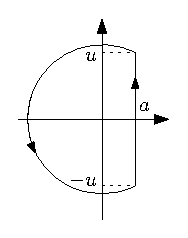
\includegraphics[scale=1.0]{05012}
Случай $b\ge1$
\end{center}
\end{wrapfigure}\par
Получаем:
$$I_0(u)=\frac{1}{2\pi i}\int\limits_{\Gamma(u)} \frac{b^s}{s^2}\,ds = \res_{s = 0}\frac{b^s}{s^2} = \res_{s=0}\frac{1+s\ln b + \ldots}{s^2} = \ln{b}.$$\par
С другой стороны,
$$I_0(u) = \underbrace{\frac{1}{2\pi i}\int\limits_{a - iu}^{a + iu}\frac{b^s}{s^2}\,ds}_{I_1(u)} +
\underbrace{\frac{1}{2\pi i}\int\limits_{\Gamma_1(u)}\frac{b^s}{s^2}\,ds}_{I_2(u)},$$
где $\Gamma_1$~— дуга окружности.\par
Очевидно, $I_1(u)\xra{u\to\infty}I$.\par
Осталось проверить, что второй интеграл стремится к нулю:
$$|I_2(u)| \leqslant \frac{2\pi\sqrt{a^2 + u^2}}{2\pi}\frac{b^a}{a^2 + u^2}\xrightarrow{u \to \infty} 0.$$\par
\begin{wrapfigure}{r}{80pt}
\begin{center}
\vskip -30pt
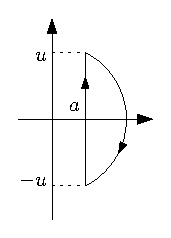
\includegraphics[scale=1.0]{05013}
Случай $0 < b < 1$
\end{center}
\end{wrapfigure}
\pt{2} При $0 < b <1$ замыкаем контур частью той же окружности, только лежащей в правой полуплоскости.\par
Ни внутри области, ограничиваемой контуром интегрирования, ни на самом контуре подынтегральная функция особых точек не имеет, поэтому
$$\hat{I_0}(u) = \frac{1}{2\pi i}\int\limits_{\hat{\Ga}(u)} \frac{b^s}{s^2}\,ds = 0.$$\par
Вместе с тем ($\hat{\Ga}_1$~— дуга окружности) $$\hat{I_0}(u)=\frac{1}{2\pi i}\int\limits_{a - iu}^{a + iu}\frac{b^s}{s^2}\,ds+
\frac{1}{2\pi i}\int\limits_{\hat{\Ga}_1(u)}\frac{b^s}{s^2}\,ds,$$
и аналогично первому пункту первый интеграл сходится к $I$, а второй~— к $0$.
\end{proof}
\begin{stm}
Для $\om(x)$ при $x\ge2$ верна формула
$$\om(x)=\frac{1}{2\pi i}\int\limits_{2 - i\infty}^{2 + i\infty}\left(-\frac{\zeta '(s)}{\zeta(s)}\right) \cdot \frac{x^s}{s^2}\,ds.$$
\end{stm}
\begin{note}
Именно этим и удобна функция $\om(x)$~— в аналогичной формуле для $\psi(x)$ в знаменателе стоит $s$ не во второй, а в первой степени, что влечет за собой отсутствие абсолютной сходимости интеграла и, таким образом, необходимость рассматривать главное значение, интегрировать не по всей прямой, что неизбежно выливается в значительные технические сложности.
\end{note}
\begin{proof}
Действовать будем так:
$$I = \frac{1}{2\pi i}\int\limits_{2 - i\infty}^{2 + i\infty} \left(\sum\limits_{n=1}^{\infty} \frac{\Lambda(n)}{n^s}\right) \frac{x^s}{s^2} \,ds\eqvl{I}{10} \sum\limits_{n=1}^{\infty} \Lambda(n) \frac{1}{2\pi i} \int\limits_{2 - i\infty}^{2 + i\infty} \frac{(\frac{x}{n})^s}{s^2}\,ds \eqvl{II}{10}\sum\limits_{n\leqslant x} \Lambda(n) \ln\frac{x}{n} = \omega(x).$$\par
Нужно обосновать два равенства~— I и II.\par
\pt{1} С I все просто~— мы меняем здесь местами сумму и интеграл, и действительно можем это делать, потому как
$$\left|-\frac{\zeta '(s)}{\zeta (s)} \cdot\frac{x^2}{s^2}\right| \leqslant \frac{C\sqrt{t} x^2}{t^2 + 4},$$
откуда и следует необходимая нам абсолютная сходимость интеграла.

\begin{note}
У подобной оценки для функции $\psi$ в знаменателе стоит $\sqrt{t^2+4}$, поэтому абсолютная сходимость отсутствует.\par
\end{note}\par
\pt{2} Разберемся с II. Выберем $N > x$ и разобьем сумму на две:
$$\sum\limits_{n=1}^{\infty} \Lambda(n) \frac{1}{2\pi i} \int\limits_{2 - i\infty}^{2 + i\infty} \frac{(\frac{x}{n})^s}{s^2}\,ds
=\sum\limits_{n=1}^{N}\ldots + \underbrace{\sum\limits_{n=N+1}^{\infty}\ldots}_{R_N(s)}\eqvl{\text{лемма }\ref{lemma_for_om_formula}}{40}\om(x)+R_N(s).$$\par
Остается показать, что $R_N(s)\xra{n\to\infty}0$.\par
Вернем сумму под интеграл:
$ R_N(s) = \frac{1}{2\pi i}\int\limits_{2 - i\infty}^{2 + i\infty} \left(\sum\limits_{n = N + 1}^{\infty} \frac{\Lambda(n)}{n^s}\right) \frac{x^s}{s^2}\,ds,$ получаем оценку
$$|R_N(s)| \leqslant \frac{1}{2\pi}\left(\sum\limits_{n = N + 1}^{\infty}\frac{\ln n}{n^2}\right) x^2 \left(\int\limits_{-\infty}^{+\infty} \frac{dt}{t^2 + 4}\right) = \frac{x^2}{2\pi} \frac{\pi}{2} \sum\limits_{n = N+1}^{\infty} \frac{\ln n}{n^2} \xrightarrow{N\to\infty} 0.$$
\end{proof}\par

Хотим показать, что $\omega(x) \sim x$. Грубо оценивая, имеем 
$\omega(x) < Cx^2$ ($Cx^{1+\ep}$, если устремим прямую интегрирования 
к $1$)~— в любом случае хуже тривиальной оценки $\omega(x) < x\ln ^2 x$.

%\begin{note}
%С этого места лучше читать книгу Галочкина в районе 45 страницы. Когда-нибудь с учетом этого мы приведем лекцию в порядок.
%\end{note}

\subsubsection{Выделение главного члена в интегральной формуле для $\om(x)$}

Нужно, чтобы значительная часть интеграла проходила левее $\Re s=1$. Выберем путь интегрирования $\Gamma(\eta, T)$, зависящий от двух параметров $T,\,T>0$ и $\eta,\,0<\eta<1$, значение которых подберем уже по ходу доказательства.\par
\begin{wrapfigure}{r}{80pt}
\begin{center}
\vskip -20pt
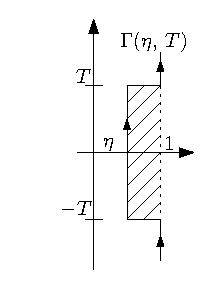
\includegraphics[scale=1.0, trim=20 0 0 0]{05021}
\end{center}
%\caption{Область интегрирования}
\end{wrapfigure}
\begin{stm} Если в заштрихованной области $\zeta(s) \not = 0$, то
$$\omega(x) = x(1 + R(x))$$ где $$R(x) = \frac{1}{2\pi i} \int\limits_{\Gamma(\eta, T)} \left(-\frac{\zeta '(s)}{\zeta (s)}\right)\frac{x^{s-1}}{s^2}\,ds.$$
\end{stm}
\begin{proof}
\begin{wrapfigure}{r}{100pt}
\begin{center}
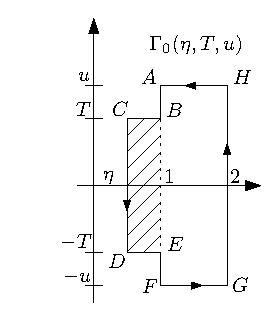
\includegraphics[scale=1.0, trim=20 0 0 0]{05022}
\end{center}
%\caption{Область интегрирования}
\end{wrapfigure}

Будем рассматривать интегралы по контуру $\Ga_0(\eta,T,u)$. Заметим, что 
в пределе (при $u\to\infty$) интеграл от функции $-\frac{\zeta '(s)}{\zeta 
(s)} \frac{x^s}{s^2}$ по пути $ABCDEF$ дает нам $-xR(x)$, а по пути $GH$~—
$\om(x)$. Сейчас мы докажем, что интеграл по всему контуру $\Ga_0$ равен $x$, 
затем~— что интегралы по перемычкам $FG$ и $HA$ равны $0$, откуда, переходя 
к пределу, получим равенство $x = \om(x) - xR(x)$.

Действительно, рассмотрим
$$I_0(u):=\frac{1}{2\pi i} \int\limits_{\Gamma_0(\eta,T,u)}
\left(-\frac{\zeta '(s)}{\zeta (s)}\right)\frac{x^{s}}{s^2}\,ds = 
\res_{s=1} \left(-\frac{\zeta '(s)}{\zeta (s)}\right)\frac{x^s}{s^2}
\eqvl{$(*)$}{10}x.$$

Почему верен переход $(*)$? Как мы знаем (формула $(\ref{36})$), $\ze(s)$ 
представима в виде $\zeta(s) \bw= \frac{1}{s-1} + f(s)$, где $f$~— 
аналитическая в области $\sigma > 0$, тогда
$$-\frac{\zeta '(s)}{\zeta (s)} = -\frac{-1/(s-1)^2 + f'(s)}{1/(s-1) + f(s)} = 
\frac{1}{s-1}\frac{1 - (s-1)^2f'(s)}{1 + (s-1)f(s)},$$
откуда следует, что функция $-\frac{\zeta '(s)}{\zeta (s)} \frac{x^s}{s^2}$
имеет в нашей области единственную особую точку $s=1$, вычет в которой равен 
$x$.

Остается показать, что интеграл по перемычкам $FG$ и $HA$ стремится к нулю 
при $u\to\infty$:
$$\left|\mp\frac{1}{2\pi i} \int\limits_{1 \pm iu}^{2\pm iu}
\left(-\frac{\zeta '(s)}{\zeta (s)}\right)\frac{x^s}{s^2}\,ds\right| \leqslant
\frac{1}{2\pi}\cdot 1\cdot c\sqrt{u}\cdot\frac{x^2}{u^2} \xra{u\to\infty} 0.$$

Значит, $\limlim_{u\to\infty}I_0(u) =x= \omega(x) - xR(x)$.
\end{proof}

\subsubsection{Доказательство асимптотического закона}

\begin{theorem}[Асимптотический закон]
%$$\lim\limits_{x\to+\infty} \frac{\pi(x) \ln(x)}{x} = 1$$
При $x\to+\infty$ 
$$
	\pi(x)\sim \frac{x}{\ln{x}}.
$$
\end{theorem}
\begin{wrapfigure}{r}{80pt}
\begin{center}
%\vskip 20pt
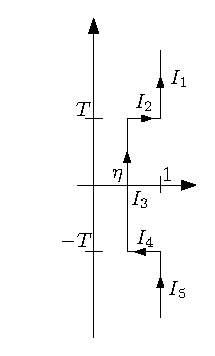
\includegraphics[scale=1.0, trim=20 0 0 0]{05024}
\end{center}
\end{wrapfigure}
%\vskip 20pt
\begin{proof}
Теперь нам достаточно доказать, что $\lim\limits_{x\to+\infty} R(x) = 0$.\par
Имеем $R(x) = I_1(x) + I_2(x) + I_3(x) + I_4(x) + I_5(x)$.\par
Сначала выбираем $T \geqslant 3$. Начнем оценивать с $I_1(x) = \frac{1}{2\pi i} \int\limits_{1 + iT}^{1 + i\infty} \left(-\frac{\zeta '(s)}{\zeta (s)}\right)\frac{x^{s-1}}{s^2}\,ds.$\par
Заметим, что $|x^{s-1}| = |x^{it}| = 1$, значит, оценка имеет вид:
$$|I_1(x)| \leqslant \frac{1}{2\pi} \int\limits_T^{+\infty} \frac{c\sqrt{t} }{1 + t^2}\cdot1\,dt < \frac{\ep}5,\text{ где }T > T_0(\ep).$$\par
Аналогично $|I_5(x)| < \ep/5$.

%\begin{wrapfigure}{r}{80pt}
%\begin{center}
%\vskip -10pt
%\includegraphics[scale=1.0, trim=20 0 0 0]{05023}
%Ука\-зан\-ная область
%\end{center}
%\end{wrapfigure}
У аналитической функции $\ze(s)$ в заштрихованной области $BCDE$ конечное число
нулей: в противном случае они имеют предельную точку, и $\ze(s)\equiv0$. 
Выберем $\eta$ как половину расстояния от $\{\si=1\}$ до ближайшего нуля.

Заметим, что благодаря такому выбору $\eta$ функция
$\left|-\frac{\zeta '(s)}{\zeta (s)} \frac{1}{s^2}\right|$ непрерывна на 
$BCDE$. Тогда найдется такая константа $M=M(T,\eta)$, что
$$\left|-\frac{\zeta '(s)}{\zeta (s)} \frac{1}{s^2}\right| \leqslant M.$$

Оценим еще пару интегралов. Рассмотрим
$I_2(x) = \frac{1}{2\pi i}\int\limits_{\eta + iT}^{1 + iT} 
\left(-\frac{\zeta '(s)}{\zeta (s)}\right) \frac{x^{s-1}}{s^2}\,ds.$ 
Для него верна оценка
$$|I_2(x)| \le \frac{1}{2\pi}\int\limits_{\eta}^{1} M x^{\si -1}\,d\si \le
\frac{1}{2\pi}\int\limits_{-\infty}^{1} M x^{\sigma -1}\,d\sigma = 
\frac{1}{2\pi}\frac{M}{\ln x} \xra{x\to\infty} 0.$$

Значит, $|I_2(x)| < \ep/5,\,|I_4(x)| < \ep/5$ при $x > x_1(\ep)$.\par
Остался последний шаг. Рассматриваем $I_3(x) = \frac{1}{2\pi i}\int\limits_{\eta - iT}^{\eta + iT} \left(-\frac{\zeta '(s)}{\zeta (s)}\right)\frac{x^{s-1}}{s^2}\,ds,$ и тогда
$$|I_3(x)| \leqslant \frac{1}{2\pi}M\cdot 2T\cdot x^{\eta-1} < \ep/5$$
при $x > x_2(\ep)$, потому как $\eta - 1 < 0$.\par
Таким образом, при $x > \max( x_1(\ep),\, x_2(\ep))$ и $T > T_0(\ep)$ получаем $$|R(x)| < \ep.$$
\end{proof}
\begin{imp}
При $n\to\infty$ $P_n \sim n\ln n$.
\end{imp}
